\documentclass[11pt]{jreport}
\usepackage{wuse_thesis}
\usepackage{indentfirst}
\usepackage{url}	% \url{}コマンド用.URLを表示する際に便利
\usepackage{xcolor}
\usepackage[dvipdfmx]{graphicx}  % ←graphicx.styを用いてEPSを取り込む場合有効にする
			% 他のパッケージ・スタイルを使う場合には適宜追加
\usepackage{tabularx}
\usepackage{listings}
\usepackage{amsmath}
\usepackage{array}

\newcommand{\todo}[1]{\colorbox{yellow}{{\bf TODO}:}{\color{red} {\textbf{[#1]}}}}  %"\todo{}"でtodoコマンド利用可
\newcommand{\change}[1]{\colorbox{green}{{\bf CHANGE}:}{\color{blue} {\textbf{[#1]}}}}  %"\change{}"でchangeコマンド利用可
\newcommand{\new}[1]{\colorbox{cyan}{{\bf NEW}:}{\color{black} {\textbf{[#1]}}}}  %"\new{}"でnewコマンド利用可
%%%%%%%%%%%%%%%%%%%%%%%%%%%%%%%%%%%%%%%%%%%%%%%%%%%%%%%%%%%%%%%%%%%%%%%%

%%
%% 主に表紙を作成するための情報
%%

%%  タイトル(修論の場合は英語表記も指定)
\title{ScratchにおいてCTスキルが向上する\\リミックス作品の分析}
%\etitle{Test\\Test\\Test}

%%  著者名(修論の場合は英語表記も指定)
\author{堀尾 桃夏}
%\eauthor{Akinori Ihara}

%% 卒業論文・修士論文(以下のどちらかを選択)
\bachelar	% 卒業論文(4年生用)

%%  学科・クラスタ
\department{システム工}
\department{デザイン情報}

%%  学生番号
\studentid{60266269}

%%  卒業年度
\gyear{2024}		% 提出年が2022年なら,2021年度

%%  論文提出日
\date{2025年2月12日}	

%%%%%%%%%%%%%%%%%%%%%%%%%%%%%%%%%%%%%%%%%%%%%%%%%%%%%%%%%%%%%%%%%%%%%%%%

\begin{document}

\maketitle

%%
%%  概要
%%
\begin{abstract}

% 本研究では,Scratchのリミックス機能におけるユーザのコンピュテーショナル・シンキング(CT)に適した作品推薦に向けて,ユーザのCTが向上するリミックス作品とは\todo{何なのかっていう言葉が気になるから考える}何なのかを示す.

% Scratchとは,プログラミング初学者向けのビジュアルプログラミング言語であり,ブロックをジグソーパズルのようにつなげることでプログラミングをすることができる.また,制作した作品をオンライン上に公開することができ,他ユーザが公開した作品を複製し,編集することができるリミックスという機能がある.従来研究により,リミックスを行うとユーザのCTが向上することが示された.本研究では,ScratchにおけるCTの評価として作品のCTスコア,ブロック数,ブロックの種類数,スプライト数を注視する.CTスコアとはDr.Scratchにより定められたスコアで,作品を7つの概念に基づいて定量的に評価した指標である.

% 仮説としてユーザのCTに適した作品をリミックスすることがより効果的ではないかと考える.しかし,現時点のScratchには作品を探す方法がキーワード検索しかなく,ユーザのCTに適した作品を探すことが困難である.従来研究では,ユーザがリミックスしたリミックス元作品の一致不一致により,ユーザ類似を抽出し,類似しているユーザがリミックスした別のリミックス元作品を推薦するという手法が提案された.しかし,この従来手法だと,類似しているユーザがいない場合に推薦することが不可能であり,ユーザのCTに適しているリミックス元作品とは異なる可能性がある.

% 本研究ではScratchのリミックス機能におけるユーザのCTに適した作品推薦に向けて,ユーザのCTとユーザのCTに影響を与えるリミックス作品の関係を調査し,分析を行った.\todo{手法,結果またはこの研究が今後の情報社会でのプログラマー育成に役立つことを書く}本研究は,Scratchにおけるリミックス機能により,ユーザの向上させたいCTを意図的に向上させることができる可能性と,リミックス元作品を推薦する際に何をベースにするべきかを示し,ユーザのCTに適したリミックス元作品推薦の実装への促進になることを期待する.

\end{abstract}

%%  目次
\tableofcontents

%%  図目次 (図目次をいれたければ以下のコメントをはずす)
%\listoffigures

%%  表目次 (表目次をいれたければ以下のコメントをはずす)
%\listoftables

\newpage
\pagenumbering{arabic}	% 以降のページ番号を算用数字に

%%%%%%%%%%%%%%%%%%%%%%%%%%%%%%%%%%%%%%%%%%%%%%%%%%%%%%%%%%%%%%%%%%%%%%%%

%%
%%  本文はここから
%%

\chapter{はじめに}

近年,日本では2020年度から小学校のプログラミング教育の必修化,2021年度から中学校の技術分野において,プログラミングに関する内容の充実,2022年度から高等学校の情報科において,共通必履修科目「情報1」の新設がされている.\cite{monkashou}しかし,指導者の情報不足や人材不足,予算不足による指導者に対する問題が複数挙げられた.\cite{monkashou2}以前からプログラミング教育に力を注いでいるアメリカでは,Scratch\footnote{https://scratch.mit.edu/}\cite{resnick2009scratch}と呼ばれるプログラミング初学者向けのビジュアルプログラミング言語を通してプログラミング教育を行っている.Scratchでは「繰り返す」などの命令処理をもつブロックを,ジグソーパズルのように組み合せて作品を完成させる.また,完成した作品はオンライン上に公開することができ,公開されている他ユーザの作品は,見る,使うだけでなく,複製し,編集することも可能である.この機能をリミックスという.

ビジュアルプログラミングは,プログラミング初学者が取り組みやすいような環境にすることと,コンピュテーショナル・シンキング(CT)\cite{wing2006computational}スキルを向上させることを目的としている.学習や操作のハードルが低く,プログラミングの入門学習として,有効である.また,バグが少なく,直観的な操作のみでプログラミングをすることができるため,ユーザが短期間で作品を完成させやすく,達成感が感じやすい.近年では,情報化社会へ進展していくにつれ,プログラマー不足が深刻な問題となっている.これらを解決する第一歩として,ビジュアルプログラミング言語の活用があげられると考える.

Scratchにおいて,作品のCTスキルを計測するためには,作品評価ツールであるDr.Scratch\cite{moreno2015dr}を使用する.Dr.Scratchとは,Morenoらによって開発されたScratch作品評価ツールであり,作品の評価を論理,制御フロー,同期,抽象化,データ表現,ユーザ対話性,並列処理の7概念に基づいて行う.また,各概念を0点から3点の,合計21点とし,CTスコアとして評価する.

従来研究でYangら\cite{10.1145/2724660.2724674}と橋谷ら\cite{橋谷直樹2022scratch},により,リミックスを行うことで,ユーザの使用するブロックの種類数とCTスコアが増加し,ユーザのCTスキルが向上することが示された.極端な難易度のものをリミックスしてもCTスキルへの効果が少なく,ユーザのCTスキルに寄与したものは,ユーザのCTスキルに適した難易度の作品のリミックスだと考える.しかし,現在のScratchでは作品を探す手段はキーワード検索のみであり,ユーザのCTスキルに適した作品を探すことは困難である.解決する手段の一つとして,ユーザのCTスキルに適したリミックス元作品の推薦が有効であり,そのためには推薦に有効な情報と基準が求められる.そこで本研究では,Scratchのリミックス機能におけるユーザのCTスキルに適した作品推薦に向けて,ユーザのCTスキルとリミックス作品の関係について分析を行う.

本研究では,Scratchのリミックス機能におけるユーザのCTスキルに適した作品推薦に向けて,以下の2つのReseach Question(RQ)に対して回答する.
\todo{要検討}
\vskip.5\baselineskip

\begin{itemize}
  \item\textbf{RQ1:ユーザのCTスコアは、他ユーザの作品をリミックスすることによって向上するか?}
  \item\textbf{RQ2:リミックスによって向上するユーザのCTスコアは,CTスコア概念による傾向があるか?}
\end{itemize}

RQ1の目的として,リミックス作品とリミックス前,リミックス後のユーザのCTスコアの分析を行い,リミックスの影響により,CTスコアが向上しているか,不変か,低下しているかを調査する.

RQ2の目的として,CTスコア概念ごとに着目し,リミックス作品とリミックス前,リミックス後のユーザのCTスコアの分析を行い,リミックスの影響により,CTスコアが向上しているか,不変か,低下しているかを調査する.

以降,本論文では,2章でScratchと従来研究について述べ,3章では使用するデータセットについて述べる.続く4章では本研究のRQの目的,分析手法,分析結果,考察を述べ,5章で妥当性の脅威を述べ,6章で本論文をまとめる.


\chapter{プログラミング初学者向け言語Scratch}\label{chap:fig-tab-exp}

\section{Scratchとは}
Scratchとは,MITメディアラボにより開発された,プログラミング初学者のCTスキルを向上させることを目的としたビジュアルプログラミング言語である.\cite{resnick2009scratch}ビジュアルプログラミングは,直観的な操作だけでプログラミングをすることができ,テキストプログラミングとは違い,エラーが起こらず,またバグも起きにくいため,プログラミング初学者が学習しやすい環境になっている.Scratchでは,図\ref{fig:scratch-edt}のように制御や演算などの命令処理をもつブロックをドラッグアンドドロップにより繋げることでプログラムを実装することができる.図\ref{fig:scratch-edt}のようにScratch3.0では作品編集画面が複数の枠に分かれており,左側にブロックパレット,中央にスクリプトエリア,右側にステージとスプライトエリアが存在する.図\ref{fig:scratch-edt}の作品例では,緑の旗を押すと,スプライトの猫が10歩進み,15度回転するという動きを10回繰り返す.2019年1月3日にリリースされたScratch3.0では,拡張機能とユーザ定義によるブロックを除いて120個のブロックが存在する.2025年1月7日時点でScratchに135,070,000名以上のユーザが登録し,164,300,000件以上の作品を公開しており,多様な作品が存在する.日本のユーザは全体の1.81%を占めており,2,300,000名以上である.Scrachでは制作した作品をオンライン上に公開することができ,他ユーザの作品を複製,編集することができるリミックスという機能がある.ユーザはオンライン上に公開された作品のプログラムを確認することができるため,実装方法を他ユーザの作品から学習することができる.本研究では,リミックス作品に注目し,他ユーザの作品がユーザのCTスキル向上に寄与する基準と情報を分析する.

\begin{itemize}
  \item ブロック

図\ref{fig:scratch-edt}のような命令処理を持つブロックのことである.また,性質によって形状や色が異なり,これらをジグソーパズルのように繋げることでプログラミングする.それぞれのブロックの形状の性質は表\ref{Block}に,色の性質は表\ref{Blockcolor}に示す.

  \item スクリプト

図\ref{fig:scratch-edt}のような複数のブロックを組み合わせてできたプログラムのことである.スクリプトの定義は,「ハットブロックから始まるもの」であり,ハットブロック以外のブロックは単独でスクリプトを構成することは不可能である.

  \item スプライト

図\ref{fig:scratch-edt}のような作品中のキャラクターなどの画像オブジェクトのことである.スプライトは,座標や音,向き,大きさ,回転,ローカル変数などを持つことができ,動きを持たせることができる.また,外部から取得してきた画像を挿入したり,Scratch内のペイントツールで描写したりすることで,スプライトの見た目を編集できる.作品の大半がスプライトを含んでいる.

\end{itemize}



%-------------------
\begin{figure}[h]
\centerline{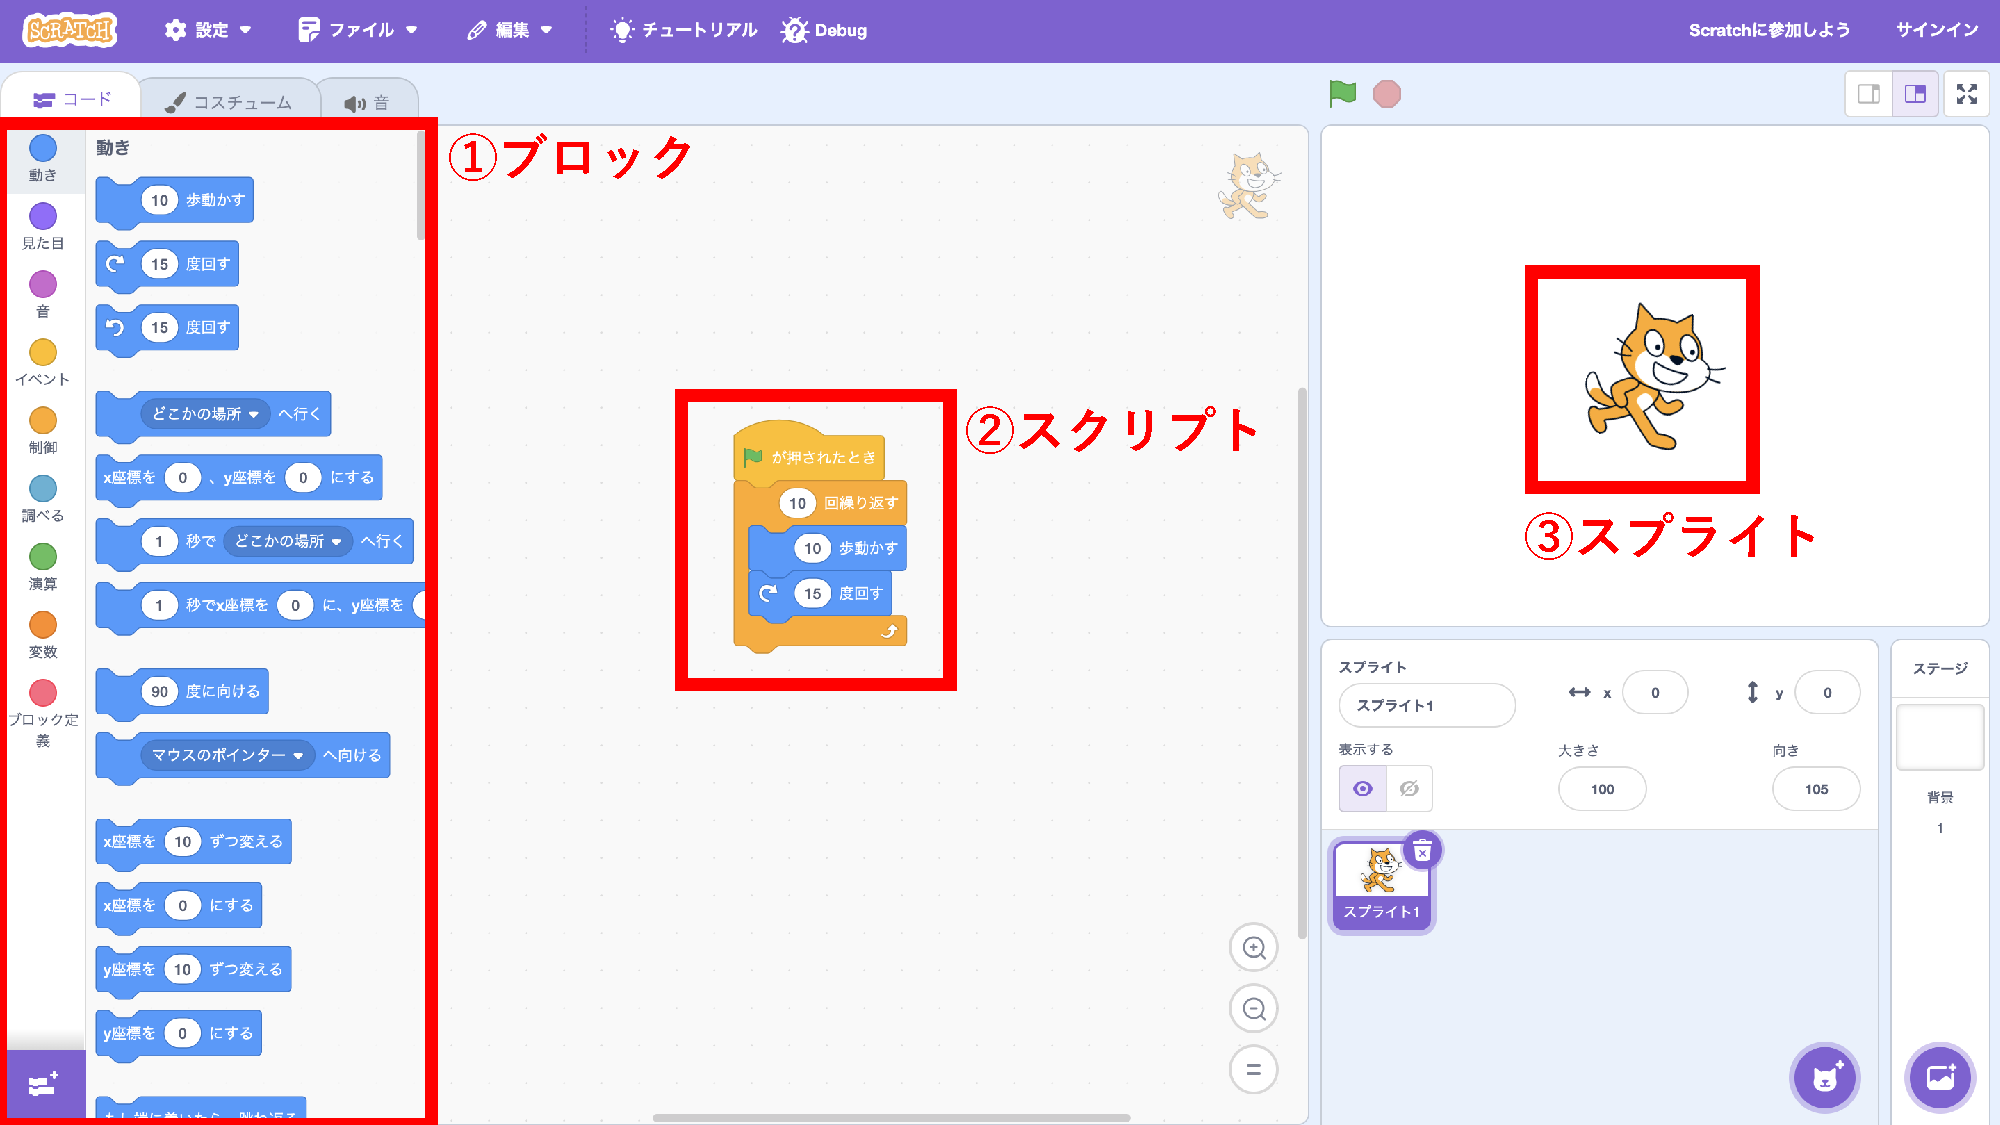
\includegraphics[width=0.8\linewidth]{@BSthesis2024_Horio/BSthesis2024_Horio_fig/scratch-edt.pdf}}
\caption{Scratch編集画面}
\label{fig:scratch-edt}
\end{figure}
%-------------------
%-------------------
\begin{table}[h]
    \centering
    \caption{ブロックの形状}
    \label{Block}
    \renewcommand{\arraystretch}{1.2}
    \scalebox{1.0}{
    \begin{tabular}{c|c|c}
    \hline
    ブロックの形状 & 名前 & 性質
    \\ \hline
    \begin{minipage}{20mm}
      \centering
      \scalebox{0.5}{
\includegraphics{@BSthesis2024_Horio/BSthesis2024_Horio_fig/hatblock.png}}
    \end{minipage}
     & ハットブロック & スクリプトを開始するブロック
    \\ \hline
    \begin{minipage}{20mm}
      \centering
      \scalebox{2.0}{
\includegraphics{@BSthesis2024_Horio/BSthesis2024_Horio_fig/stackblock.png}}
    \end{minipage}
     & スタックブロック & 各種の命令を実行するブロック
    \\ \hline
    \begin{minipage}{20mm}
      \centering
      \scalebox{2.0}{
\includegraphics{@BSthesis2024_Horio/BSthesis2024_Horio_fig/tfblock.png}}
    \end{minipage}
     & 真偽ブロック & 真または偽のどちらかの状態を表すブロック
    \\ \hline
    \begin{minipage}{20mm}
      \centering
      \scalebox{0.5}{
\includegraphics{@BSthesis2024_Horio/BSthesis2024_Horio_fig/xblock.png}}
    \end{minipage}
     & 値ブロック & 数値や文字列を返すブロック
    \\ \hline
    \begin{minipage}{20mm}
      \centering
      \scalebox{0.5}{
\includegraphics{@BSthesis2024_Horio/BSthesis2024_Horio_fig/cblock.png}}
    \end{minipage}
     & C型ブロック & 間に挟まれたブロックを制御するブロック
    \\ \hline
    \begin{minipage}{20mm}
      \centering
      \scalebox{2.0}{
\includegraphics{@BSthesis2024_Horio/BSthesis2024_Horio_fig/capblock.png}}
    \end{minipage}
     & キャップブロック & スクリプトを停止するブロック
    \\ \hline
    \end{tabular}
    }
\end{table}
%-------------------
%-------------------
\begin{table}[h]
    \centering
    \caption{ブロックの形状}
    \label{Blockcolor}
    \scalebox{1.0}{
    \begin{tabular}{c|c|c}
    \hline
    ブロックの色 & 名前 & 性質
    \\ \hline
    \begin{minipage}{20mm}
      \centering
      \scalebox{0.5}{
\includegraphics{@BSthesis2024_Horio/BSthesis2024_Horio_fig/move.png}}
    \end{minipage}
     & 動き & スプライトの動きを制御するブロック
    \\ \hline
    \begin{minipage}{20mm}
      \centering
      \scalebox{0.5}{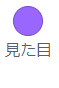
\includegraphics{@BSthesis2024_Horio/BSthesis2024_Horio_fig/look.png}}
    \end{minipage}
     & 見た目 & スプライトの見た目を制御するブロック
    \\ \hline
    \begin{minipage}{20mm}
      \centering
      \scalebox{0.5}{
\includegraphics{@BSthesis2024_Horio/BSthesis2024_Horio_fig/sound.png}}
    \end{minipage}
     & 音 & BGMやSEなどの音を制御するブロック
    \\ \hline
    \begin{minipage}{20mm}
      \centering
      \scalebox{0.5}{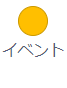
\includegraphics{@BSthesis2024_Horio/BSthesis2024_Horio_fig/event.png}}
    \end{minipage}
     & イベント & スクリプトを実行するトリガーを示すブロック
    \\ \hline
    \begin{minipage}{20mm}
      \centering
      \scalebox{0.5}{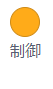
\includegraphics{@BSthesis2024_Horio/BSthesis2024_Horio_fig/seigyo.png}}
    \end{minipage}
     & 制御 & プログラムの処理の流れを制御するブロック
    \\ \hline
    \begin{minipage}{20mm}
      \centering
      \scalebox{0.5}{
\includegraphics{@BSthesis2024_Horio/BSthesis2024_Horio_fig/seach.png}}
    \end{minipage}
     & 調べる & スクリプトや操作の状態を調べるブロック
    \\ \hline
    \begin{minipage}{20mm}
      \centering
      \scalebox{0.5}{
\includegraphics{@BSthesis2024_Horio/BSthesis2024_Horio_fig/enzan.png}}
    \end{minipage}
     & 演算 & 演算を行うブロック
    \\ \hline
    \begin{minipage}{20mm}
      \centering
      \scalebox{0.5}{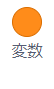
\includegraphics{@BSthesis2024_Horio/BSthesis2024_Horio_fig/hensu.png}}
    \end{minipage}
     & 変数 & 変数とリストを定義し,扱うブロック
    \\ \hline
    \begin{minipage}{20mm}
      \centering
      \scalebox{0.5}{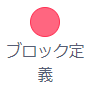
\includegraphics{@BSthesis2024_Horio/BSthesis2024_Horio_fig/teigi.png}}
    \end{minipage}
     & ブロック定義 & カスタムブロックを定義して使うことができるブロック
    \\ \hline
    \end{tabular}
    }
\end{table}
%-------------------
\section{Dr.Scratch}

Dr.ScratchとはMorenoらにより開発されたScratch作品のコンピュテーショナル・シンキング(CT)スキルを計測する支援ツールである.\cite{moreno2015dr}
CTスキルを7概念の論理,制御フロー,同期,抽象化,データ表現,ユーザ対話性,並列処理に分類しており,1概念0点から3点の合計21点で評価し,CTスコアという.各概念のスコア詳細は表\ref{CTscoreTable}に示す.また,CT習熟度がBasic,Developing,Masterの3区分に分類されており,0点から7点をBasic,8点から14点をDeveloping,15点から21点をMasterとしている.

図\ref{fig:scratch-edt}の作品をDr.Scratchを利用し,評価した場合,図\ref{fig:DrScratchgamen}のようになる.左側に合計スコア,CT習熟度が表示され,右側に,CTスコアの概念ごとに獲得することができたスコアが表示される.図\ref{fig:scratch-edt}の作品では,指定回数の繰り返しブロックを使用しているため,フロー制御が2点,緑の旗ブロックを使用しているため,ユーザ対話性が1点,オブジェクトのプロパティを編集しているため,データ表現が1点獲得している.

本研究では,Dr.ScratchによるScratch作品評価スコアのCTスコアを用いて,ユーザのCTスキルとリミックス作品の難易度を計測する,

%-------------------

\begin{table}[h]
    \centering
    \caption{CTスコア概念\cite{橋谷直樹2022scratch}}
    \label{CTscoreTable}
    \scalebox{0.7}{
    \begin{tabular}{c|c|c|c|c}
    \hline
    CTスキルの概念 & 0点 & 1点 & 2点 & 3点
    \\ \hline
    抽象化 & - &
    \begin{tabular}{c}
    2つ以上の\\スクリプトを使用
    \end{tabular}
    & 定義ブロックを使用 & クローンブロックを使用
    \\ \hline
    並列 & - & 
    \begin{tabular}{c}
    緑の旗ブロックを\\2個以上使用 
    \end{tabular}
    & 
    \begin{tabular}{c}
    オブジェクトへのクリックにより\\2つ以上のスクリプトを\\同時に実行する機能を実装
    \end{tabular}
    & 
    \begin{tabular}{c}
    イベント動作により\\2つ以上のスクリプトを\\同時に実行する機能を実装
    \end{tabular}
    \\ \hline
    論理 & - & Ifブロックを使用 & If elseブロックを使用 & 論理演算ブロックを使用
    \\ \hline
    同期 & - & 待機ブロックを使用 &
    \begin{tabular}{c}
    メッセージ受信により\\プログラムを停止する機能を実装
    \end{tabular}
    &
    \begin{tabular}{c}
    指定条件を満たすまで\\プログラムを停止する処理を実装
    \end{tabular}
    \\ \hline
    フロー制御 & - &
    \begin{tabular}{c}
    2個以上の処理ブロックを\\連結して使用
    \end{tabular}
    &
    \begin{tabular}{c}
    指定回数/回数無制限の\\繰り返しブロックを使用
    \end{tabular}
    &
    \begin{tabular}{c}
    指定条件までの\\繰り返しブロックを使用
    \end{tabular}
    \\ \hline
    ユーザ対話性 & - & 緑の旗ブロックを使用 &
    \begin{tabular}{c}
    ユーザの入力を伴う\\ブロックを使用
    \end{tabular}
    &
    \begin{tabular}{c}
    マイクやビデオなどの\\作用を伴うブロックを使用
    \end{tabular}
    \\ \hline
    データ表現 & - &
    \begin{tabular}{c}
    オブジェクトの\\プロパティを編集
    \end{tabular}
    & 変数ブロックを使用 & リスト変数ブロックを使用
    \\ \hline
    \end{tabular}
    }
\end{table}

%-------------------
%-------------------
\begin{figure}[h]
\centerline{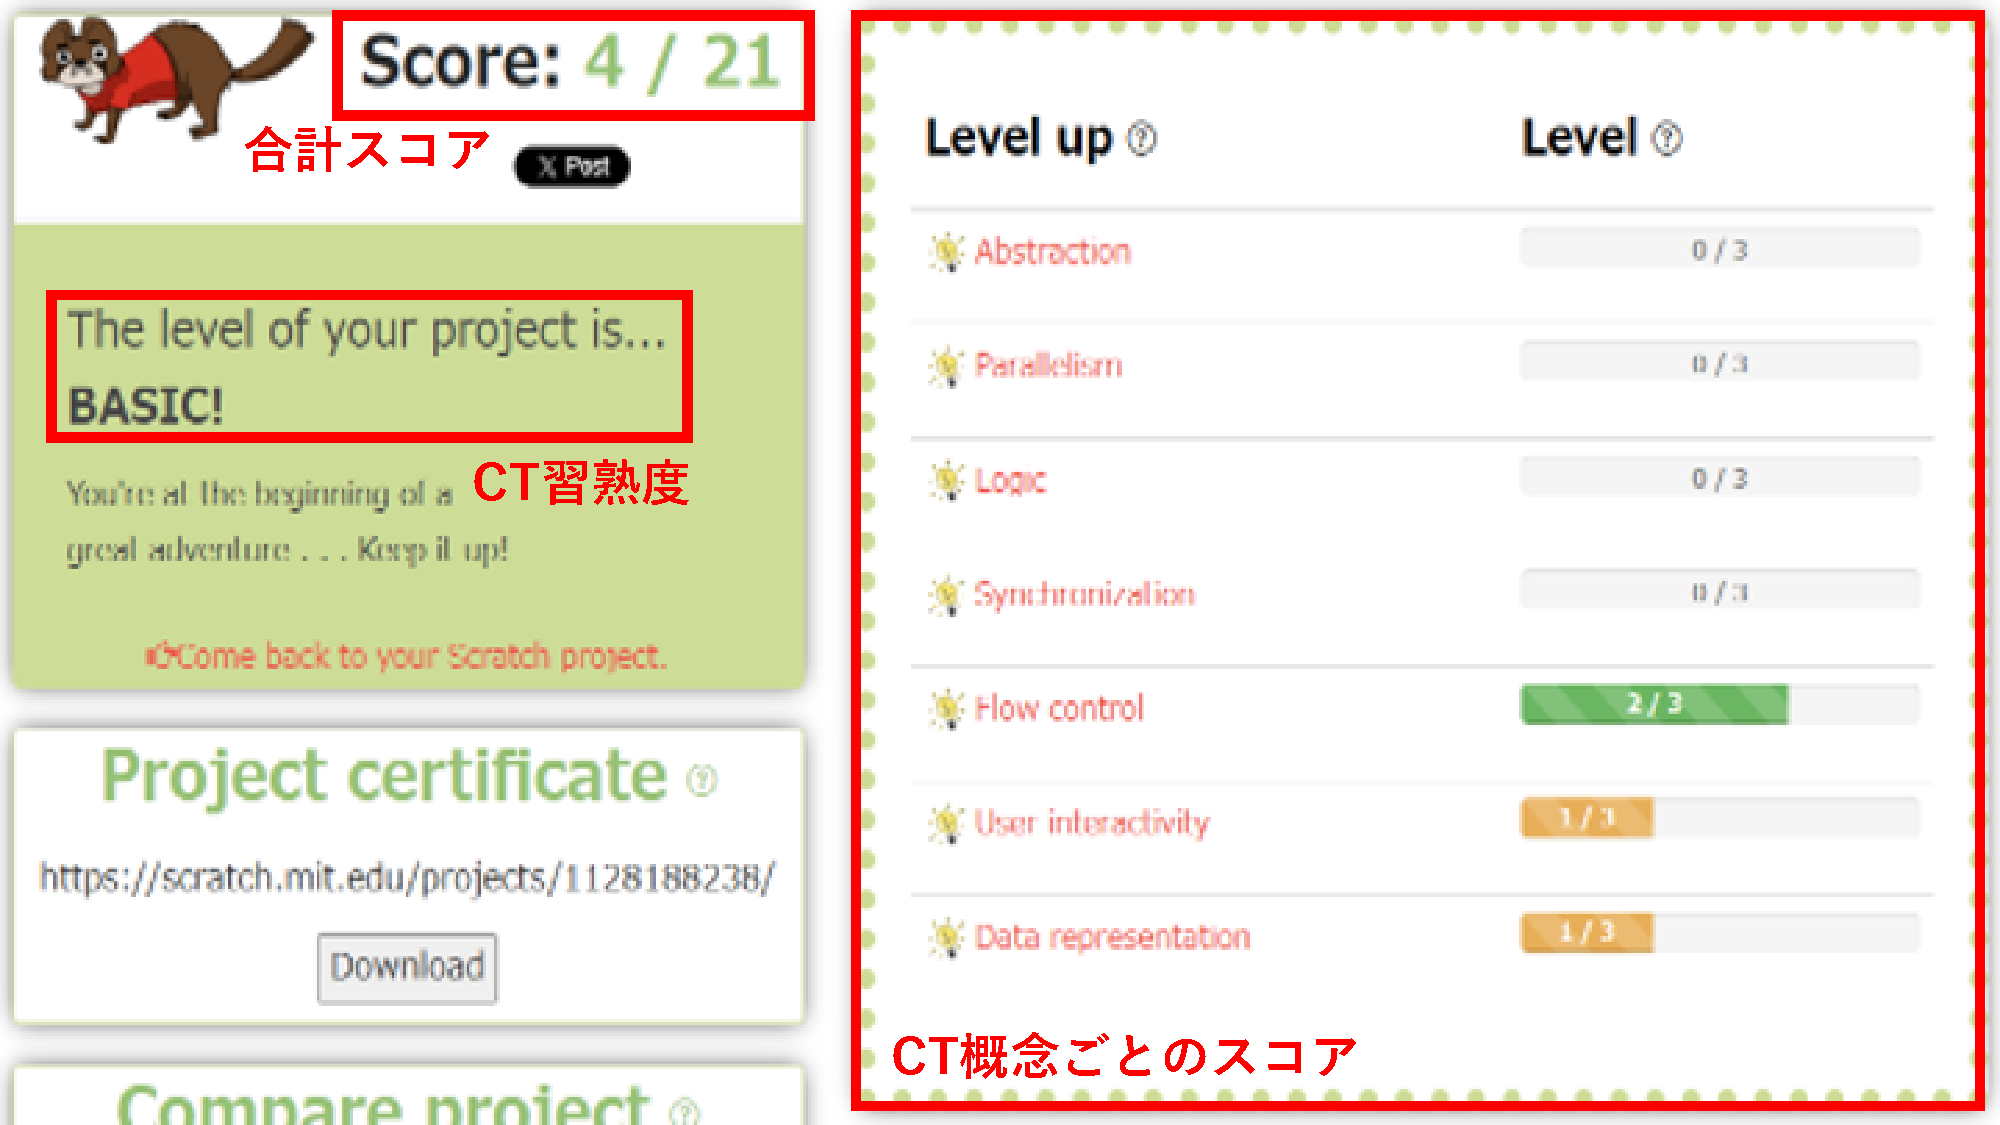
\includegraphics[width=1.0\linewidth]{@BSthesis2024_Horio/BSthesis2024_Horio_fig/DrScratchgamen.pdf}}
\caption{Dr.Scratchの評価画面}
\label{fig:DrScratchgamen}
\end{figure}
%-------------------


\section{従来研究}
Yangら\cite{10.1145/2724660.2724674}と橋谷ら\cite{橋谷直樹2022scratch}はリミックスがユーザのCTスキルにどのように影響するのかを調査し,リミックスすることで,CTスコアが向上すること,また,使用するブロックの種類数が増加することがわかった.しかし,必ず向上するわけでなく,リミックスを行うことで,CTスキルが向上した割合は示されていない.

Fesakisらはリミックス作品元の協調性フィルタリングによるユーザ類似度でリミックス作品を推薦するという手法を提案した.\cite{fesakis2009proposing}
類似性を測定することができるJaccard係数を使用し,同じ作品をリミックスしているかの一致不一致に重みづけを行い,多次元尺度構成法を用いることで類似関係を視覚化し,類似しているユーザを見つけ出した.
例えば,ユーザAとユーザBが類似しているとなった際に,ユーザAがリミックスした作品かつ,ユーザBがリミックスしたことのない作品をユーザBに推薦するという手法である.
リミックスによるCTスコア獲得にユーザのCTスキルが大きく関係しているならば,従来手法は非常に効果的だと考える.しかし,従来手法では,類似したユーザがいない場合に推薦することが不可能であることと,CTスキル向上に寄与しない作品まで推薦することが考えられる.


\section{動機}
近年,日本では2020年度から小学校のプログラミング教育の必修化,2021年度から中学校の技術分野において,プログラミングに関する内容の充実,2022年度から高等学校の情報科において,共通必履修科目「情報1」の新設がされている.\cite{monkashou}しかし,指導者の情報不足や人材不足,予算不足による指導者に対する問題が複数挙げられた.\cite{monkashou2}

また,従来研究によりScratchにおけるリミックスが,ユーザのCTスキル向上に有効だと示された.極端な難易度のものをリミックスしてもCTスキルへの効果が少なく,ユーザのCTスキルに寄与したものは,ユーザのCTスキルに適した難易度の作品のリミックスだと考える.しかし,現在のScratchでは作品を探す手段はキーワード検索のみであり,ユーザのCTスキルに適した作品を探すことは困難である.

指導者不足の問題とScratchにおける作品検索問題を解決する有効な手段として,Scratchにおけるリミックス元作品の推薦が挙げられる.推薦のためには有効な情報と基準が求められる.そこで本研究では,Scratchのリミックス機能におけるユーザのCTスキルに適した作品推薦に向けて,ユーザのCTスキルとリミックス作品の関係について分析を行う.

\section{リサーチクエスチョン}
\todo{要検討}
以下のRQの目的について説明をする.
\begin{itemize}
  \item RQ1:ユーザのCTスコアは、他ユーザの作品をリミックスすることによって向上するか?
  \item RQ2:リミックスによって向上するユーザのCTスコアは,CTスコア概念による傾向があるか?
\end{itemize}

RQ1の目的として,リミックス作品とリミックス前,リミックス後のユーザのCTスコアの分析を行い,リミックスの影響により,CTスコアが向上しているか,不変か,低下しているかを調査する.
RQ2の目的として,CTスコア概念ごとに着目し,リミックス作品のCTスコアとリミックス前,リミックス後のユーザのCTスコアの分析を行い,リミックスの影響により,CTスコアが向上しているか,不変か,低下しているかを調査する.
詳細については4章で述べる.

\chapter{ケーススタディ}

\section{概要}
本研究では,ユーザのCTスキルと作品の関係を分析するため,リミックス前作品,リミックス元作品,リミックス作品,リミックス後作品を重視する.以下で,各作品の定義を詳しく述べる.
\begin{itemize}
  \item リミックス前作品
  
  対象のリミックス作品より前に制作したオリジナル作品のうち,獲得したCTスコアが最も高い作品.リミックス前作品のCTスコアを,リミックス前のユーザのCTスキルとする.
  
  \item リミックス元作品
  
  対象のリミックス作品のリミックスを行う前の状態の作品.
  
  \item リミックス作品
  
  対象のリミックス作品.

  \item リミックス後作品
  
  対象のリミックス作品より後に制作した直近のオリジナル作品3件以下のうち,獲得したCTスコアが最も高い作品.リミックス後作品のCTスコアを,リミックス後のユーザのCTスキルとする.
  
\end{itemize}
リミックス前作品,リミックス元作品,リミックス作品,リミックス後作品のそれぞれの作品のCTスコアを元に,議論を進める.

\section{データセット}
データはScratch上に公開されているScratch3.0以降の作品をScratchAPI\footnote{\url{https://ja.scratch-wiki.info/wiki/Scratch_API_(2.0)}}により収集した.
オリジナル作品,リミックス作品を含め,20作品以上これまでに制作したことがあり,リミックスを行ったことがあるユーザを対象とする.合計7,551人のユーザの136,283件の作品をデータとして用いる.その中に,オリジナル作品は89,226件,リミックス作品は47,057件ある.また,リミックス作品について,リミックス元作品のデータ取得も行った.リミックス元作品がScratch3.0より前のものや,非公開になっているものがあり,取得できないリミックス元作品は排除し,取得できたリミックス元作品は22,271件ある.
%-------------------
\begin{table}[t]
    \centering
    \caption{各データセットの数}
    \label{CTscoreTable}
    \scalebox{1.0}{
    \begin{tabular}{c|c}
    \hline
    データセット & 件数
    \\ \hline
    オリジナル作品 & 89,226
    \\ \hline
    リミックス作品 & 47,057
    \\ \hline
    リミックス元作品 & 22,271
    \\ \hline
    \end{tabular}
    }
\end{table}
%-------------------
\chapter{RQ1:ユーザのCTスコアは、他ユーザの作品をリミックスすることによって向上するか?}

\section{概要}
リミックスすることで,ユーザのCTスコアが向上しているかを調査する.従来研究により,リミックスを行うことで,CTスコアが向上することは示されたが,必ず向上するわけでなく,実際に向上しているユーザの割合は示されていない.また,リミックスのみの影響ではなく,オリジナル作品の制作を重ねることで向上している可能性がある.そのため,リミックスを行うことで,CTスコアが向上しているか,不変か,低下しているかをリミックス前のCTスコアごとに調査する.

\section{分析手法}
分析手法として,箱ひげ図とヒストグラムにより視覚化を行うことで,ユーザのCTスコアとリミックスによる関係を発見する.使用するデータは,データセットのリミックス前作品,リミックス元作品,リミックス後作品である.縦軸をリミックス前作品のCTスコアとリミックス元作品のCTスコアの差とし,横軸をリミックス前作品のCTスコアとする.横軸では,リミックス前作品のスコアごとにリミックス前作品のCTスコアとリミックス後作品のCTスコアを比較し,上がったもの,変わらなかったもの,下がったものの3つを出力する.
検定として,CTスコアが上がったものと下がったものの2群に対し,マンホイットニーのU検定を用い,有意差の取得を行う.

\section{分析結果}


%-------------------
\begin{figure}[h]
\centerline{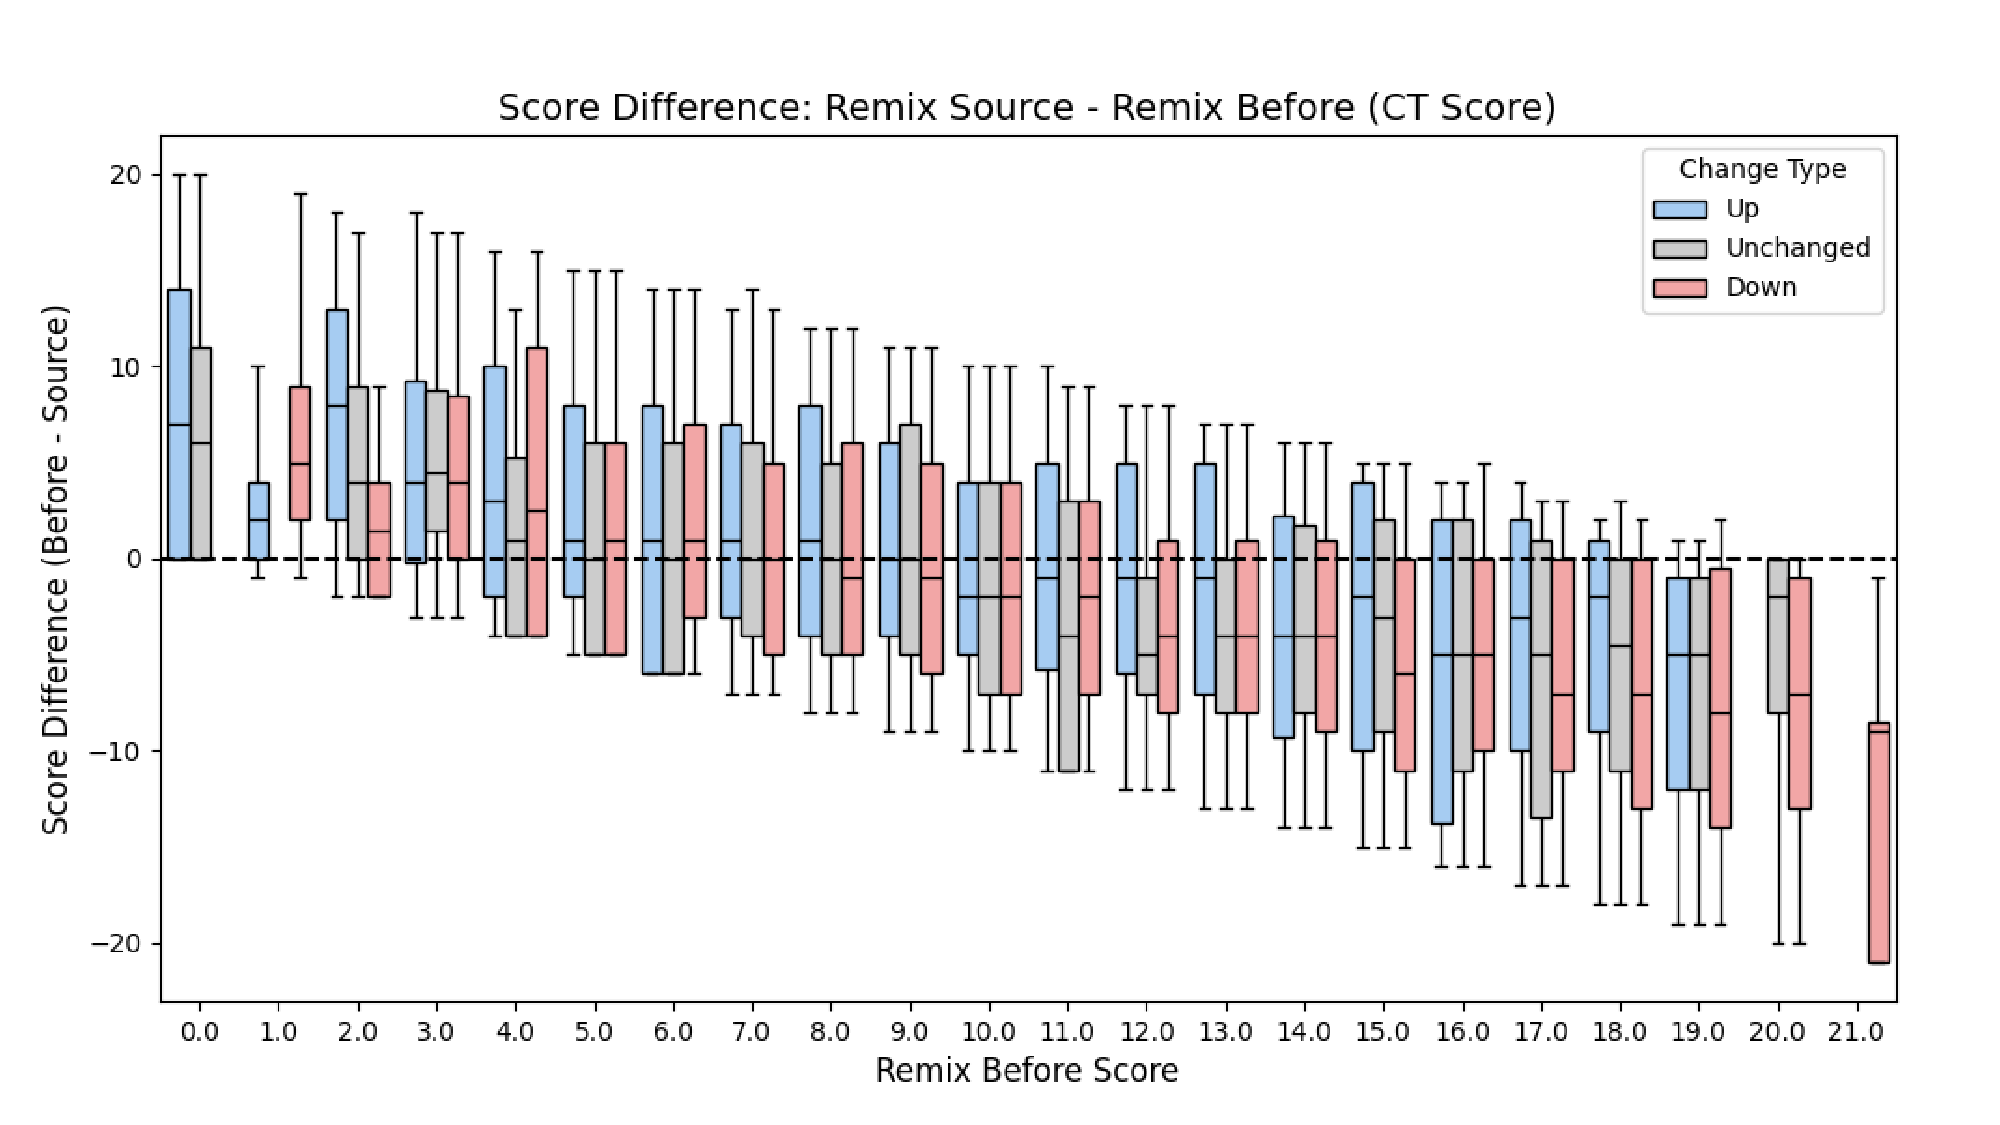
\includegraphics[width=1.0\linewidth]{@BSthesis2024_Horio/BSthesis2024_Horio_fig/CTscore-boxplot.pdf}}
\caption{ユーザのCTスコアごとのリミックス元作品のCTスコア}
\label{fig:CTscore-boxplot}
\end{figure}
%-------------------
%-------------------
\begin{figure}[h]
\centerline{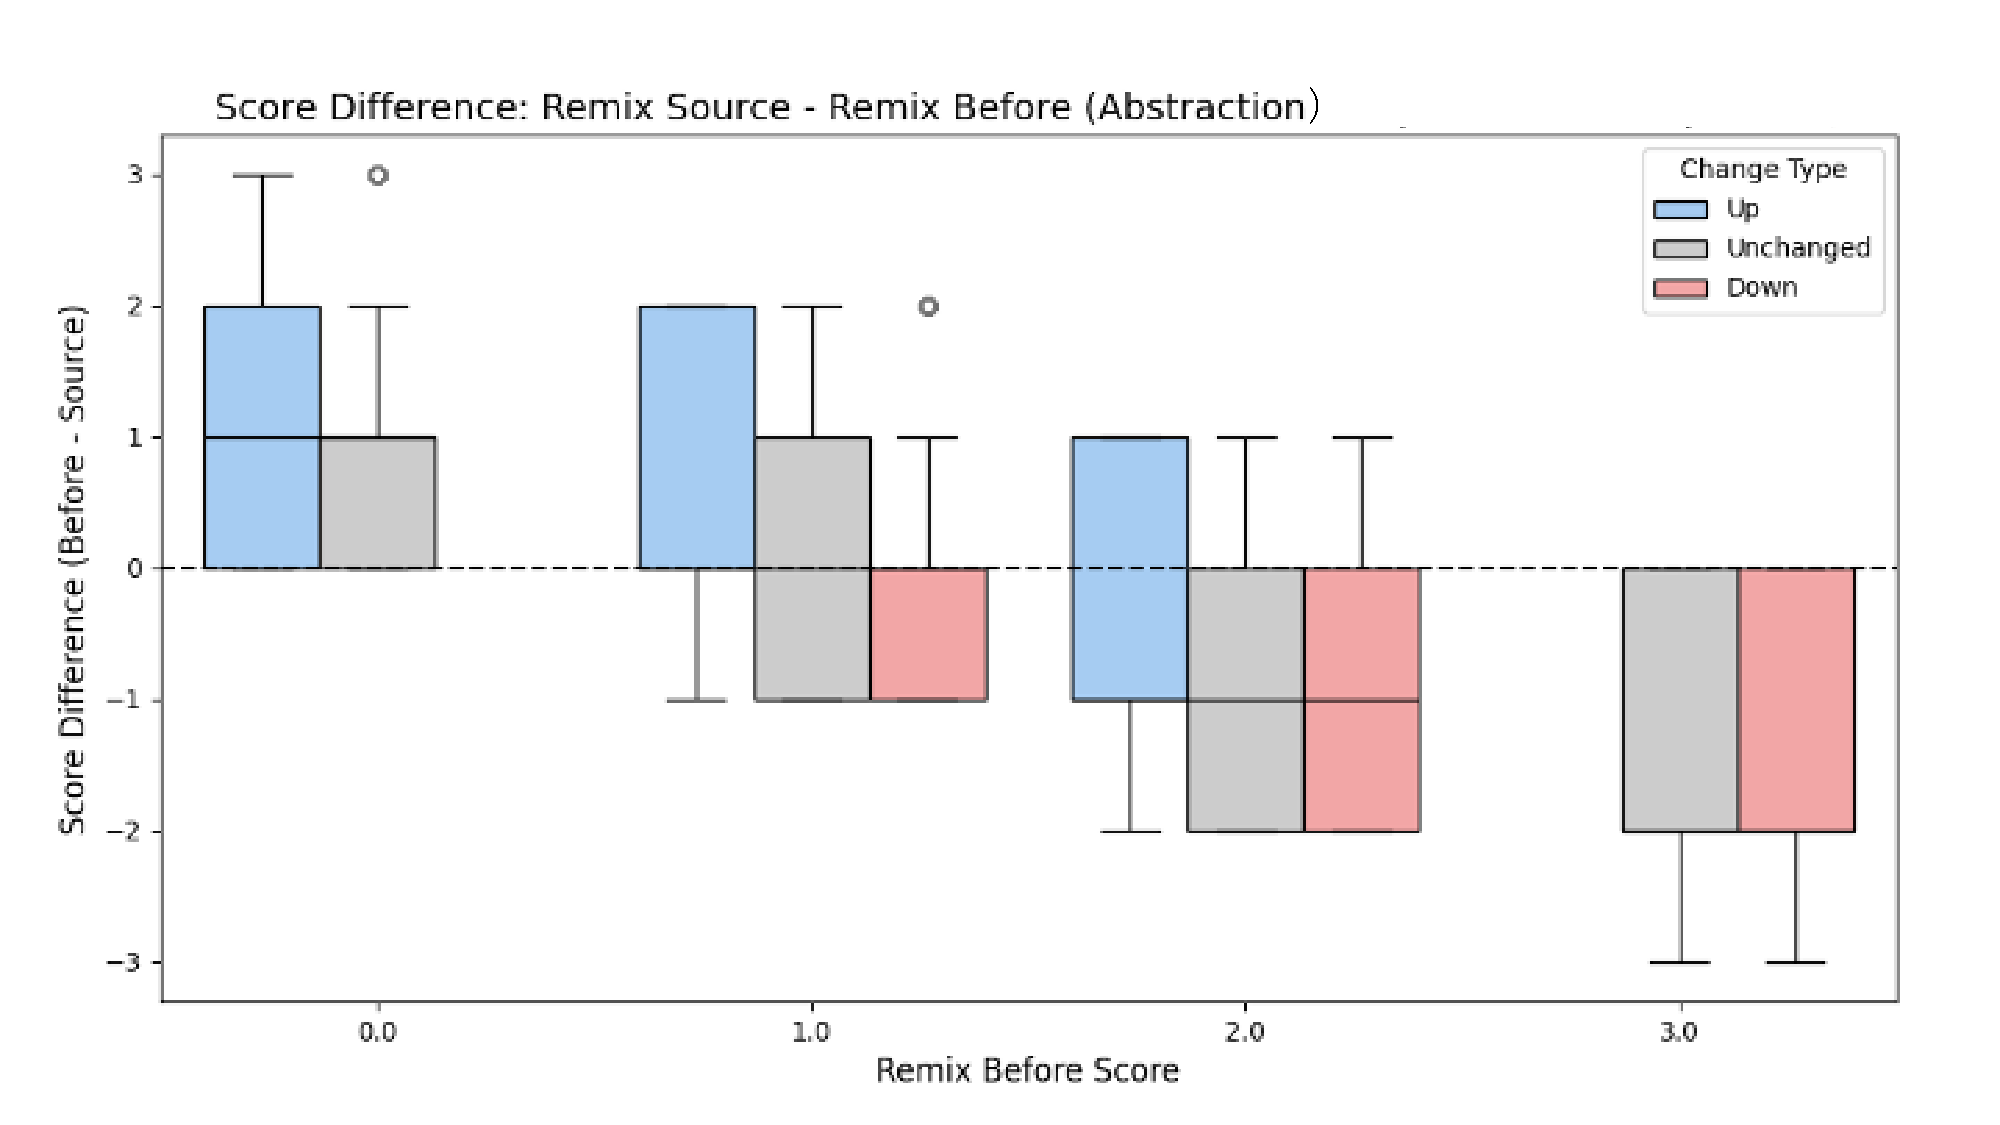
\includegraphics[width=0.7\linewidth]{@BSthesis2024_Horio/BSthesis2024_Horio_fig/Abstraction-boxplot.pdf}}
\caption{ユーザの抽象化のスコアごとのリミックス元作品の抽象化のスコア}
\label{fig:Abstraction-boxplot}
\end{figure}
%-------------------
%-------------------
\begin{figure}[h]
\centerline{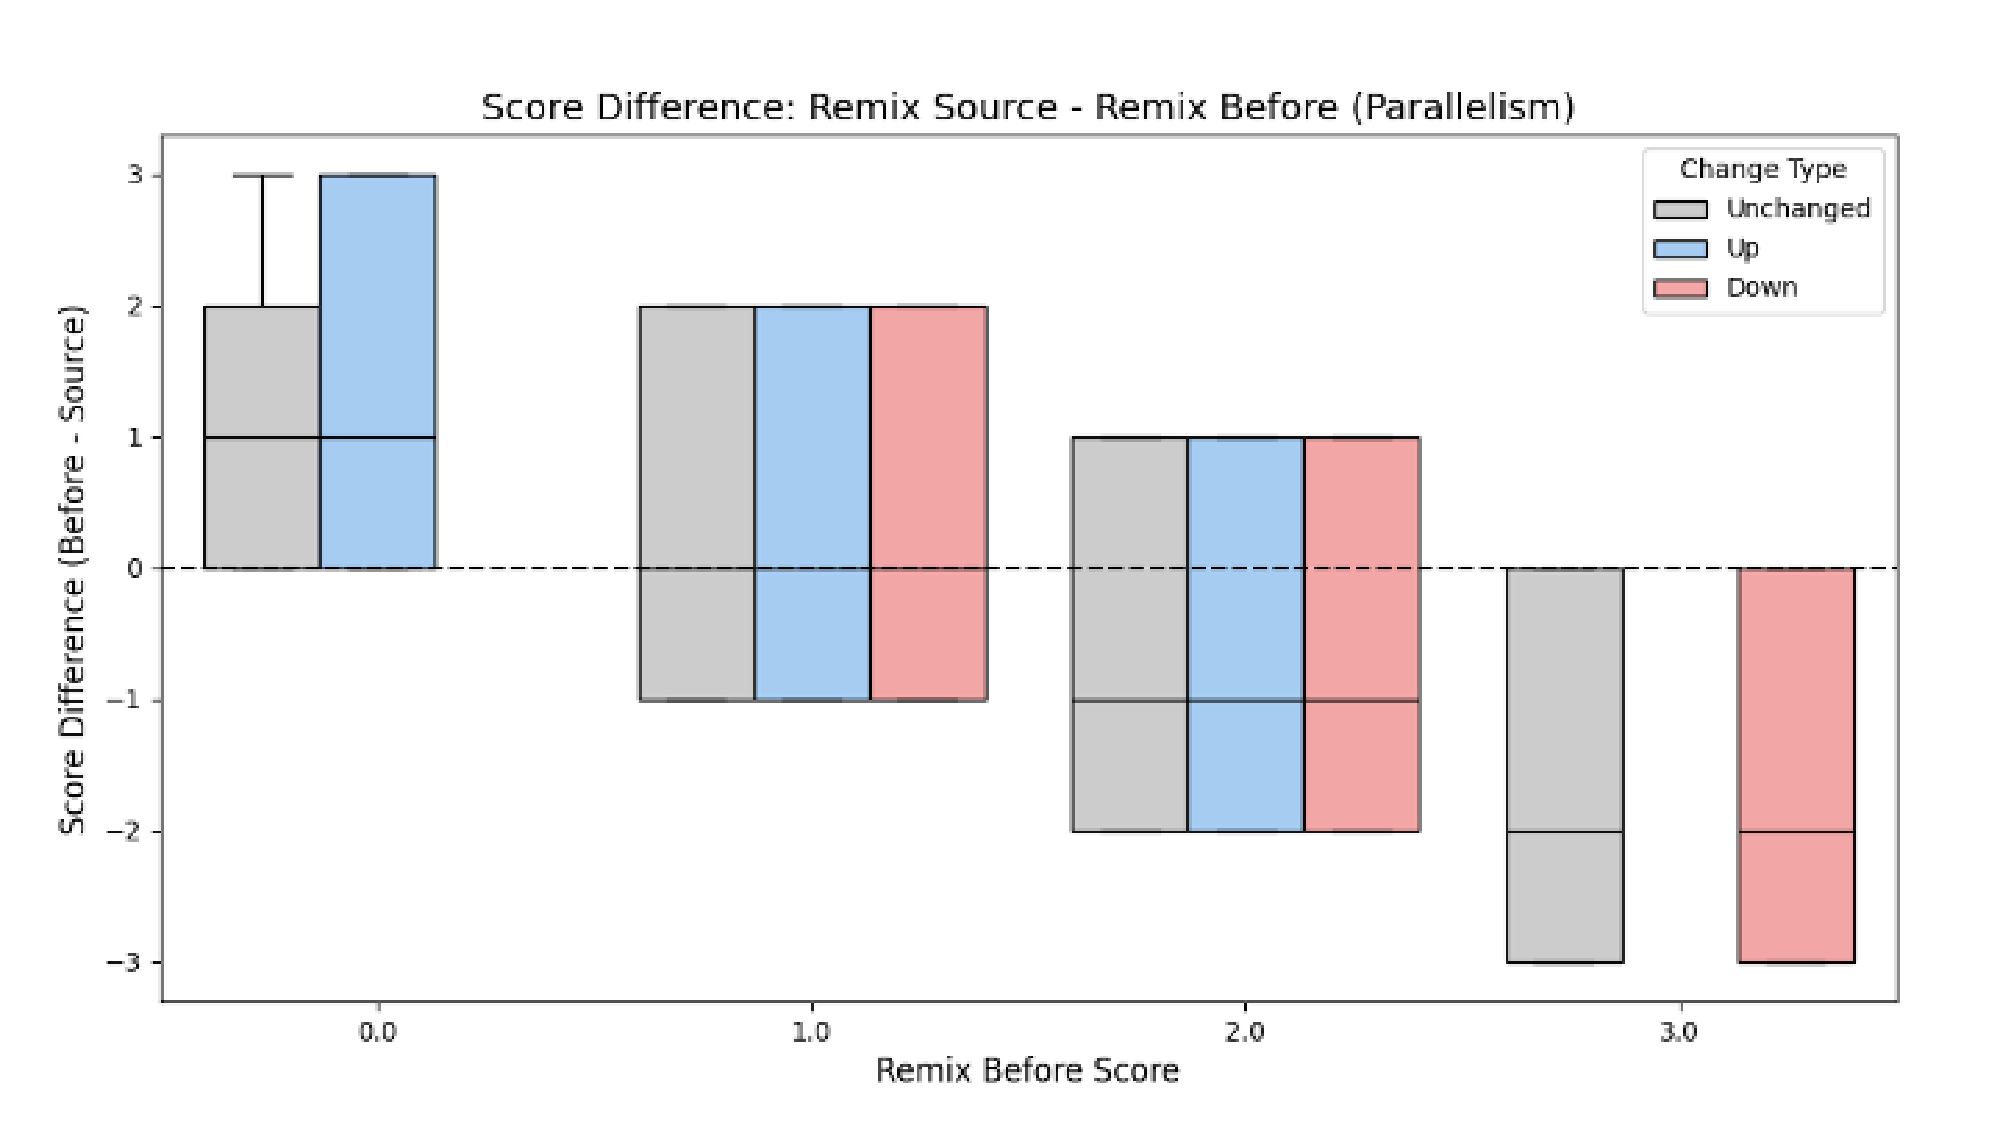
\includegraphics[width=0.7\linewidth]{@BSthesis2024_Horio/BSthesis2024_Horio_fig/Parallelism-boxplot.pdf}}
\caption{ユーザの並列スコアごとのリミックス元作品の並列スコア}
\label{fig:Parallelism-boxplot}
\end{figure}
%-------------------
%-------------------
\begin{figure}[h]
\centerline{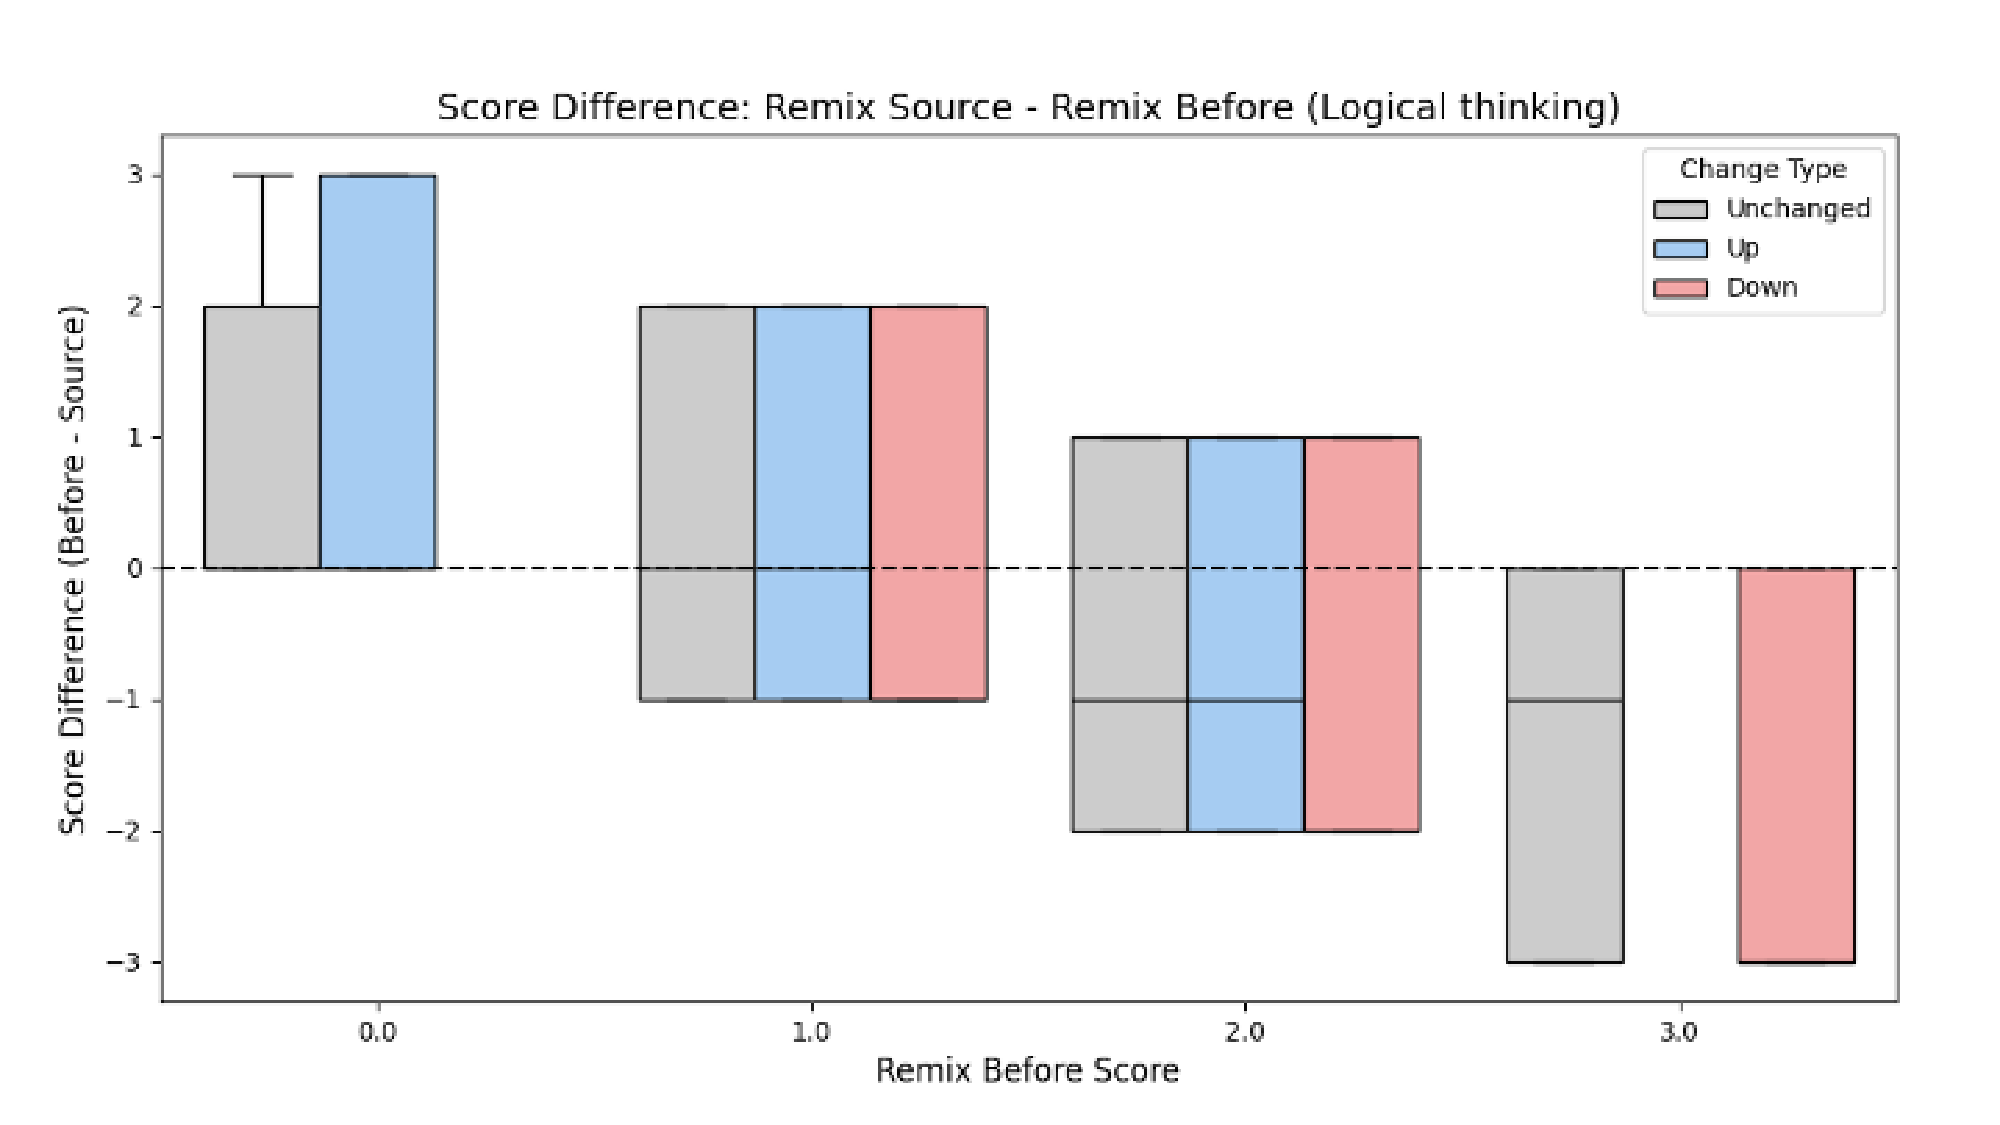
\includegraphics[width=0.7\linewidth]{@BSthesis2024_Horio/BSthesis2024_Horio_fig/Logicalthinking-boxplot.pdf}}
\caption{ユーザの論理スコアごとのリミックス元作品の論理スコア}
\label{fig:Logicalthinking-boxplot}
\end{figure}
%-------------------
%-------------------
\begin{figure}[h]
\centerline{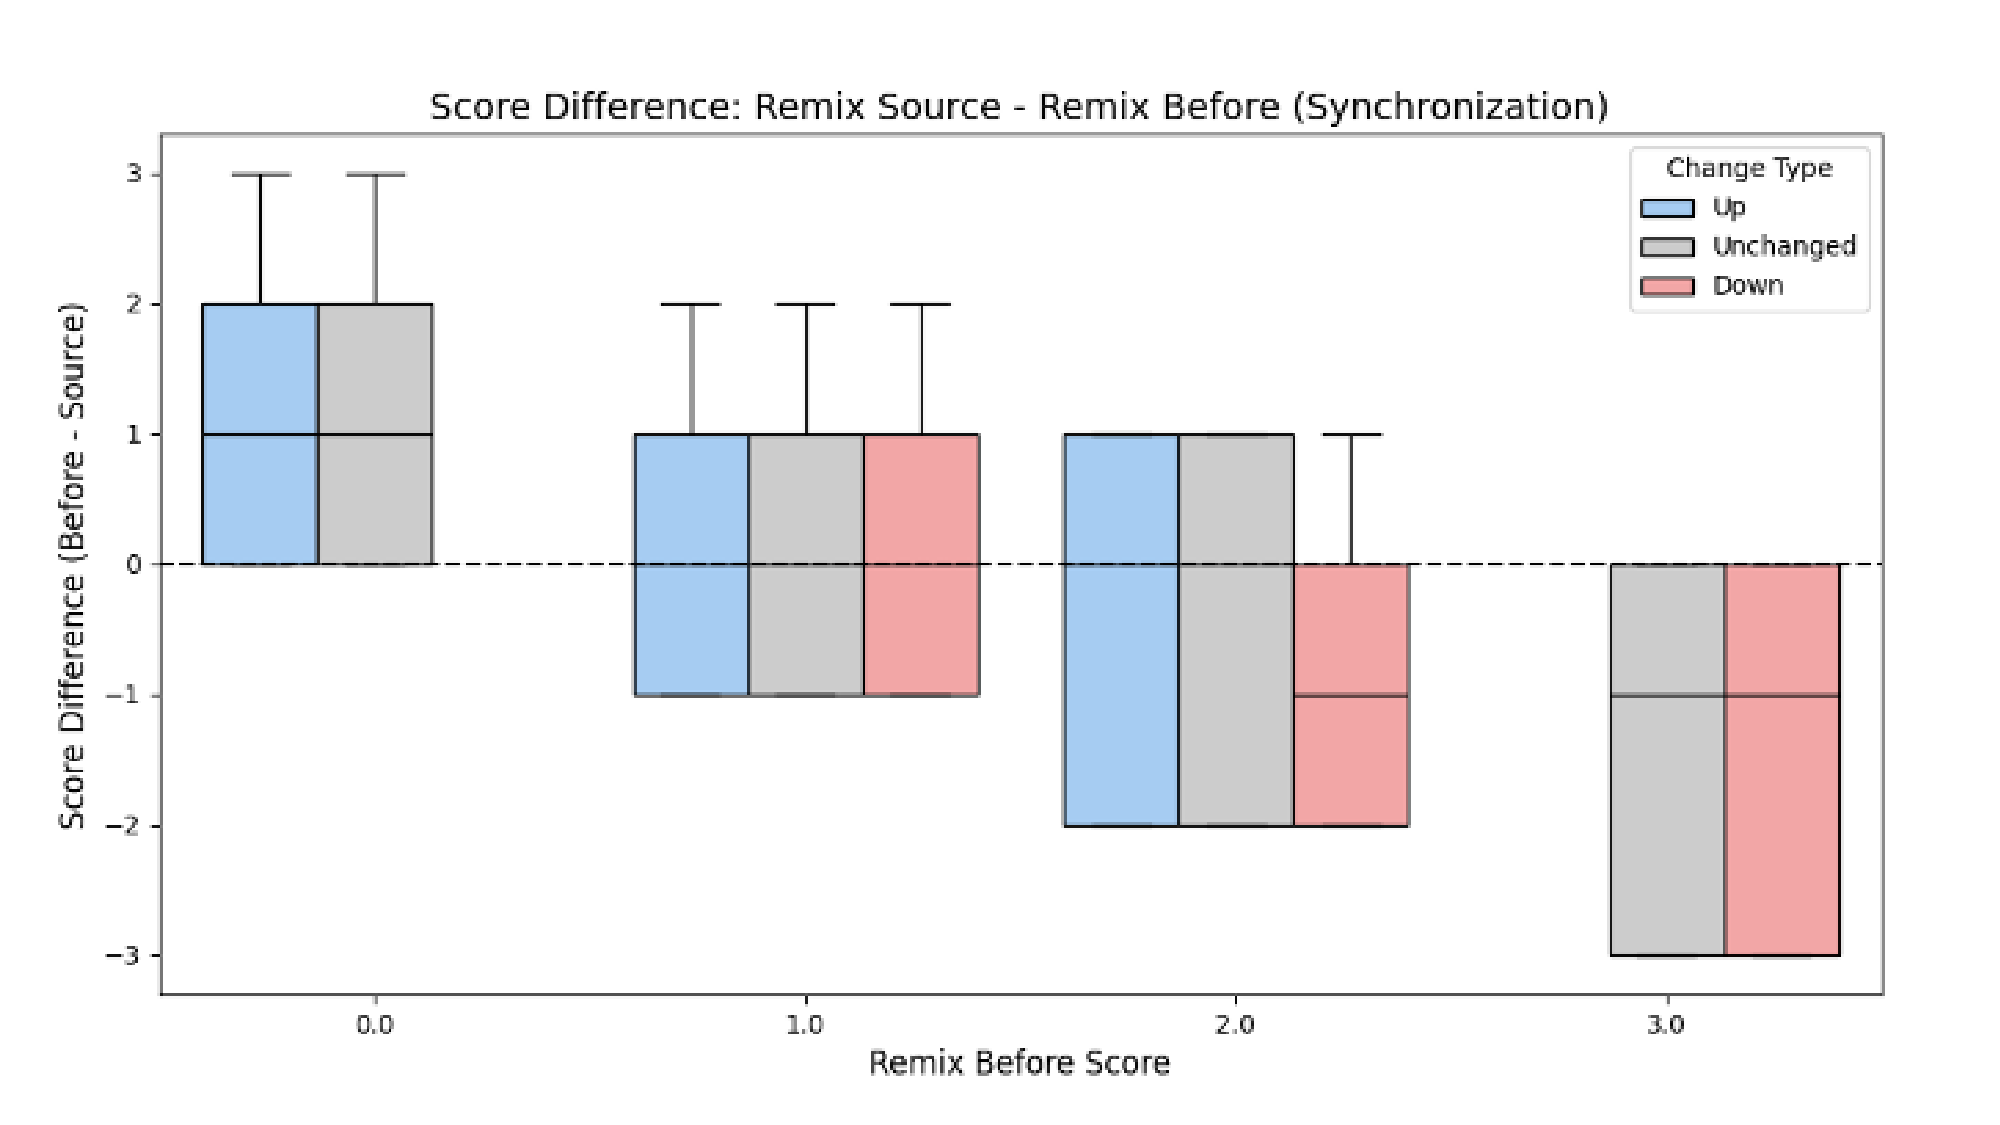
\includegraphics[width=0.7\linewidth]{@BSthesis2024_Horio/BSthesis2024_Horio_fig/Synchronization-boxplot.pdf}}
\caption{ユーザの同期スコアごとのリミックス元作品の同期スコア}
\label{fig:Synchronization-boxplot}
\end{figure}
%-------------------
%-------------------
\begin{figure}[h]
\centerline{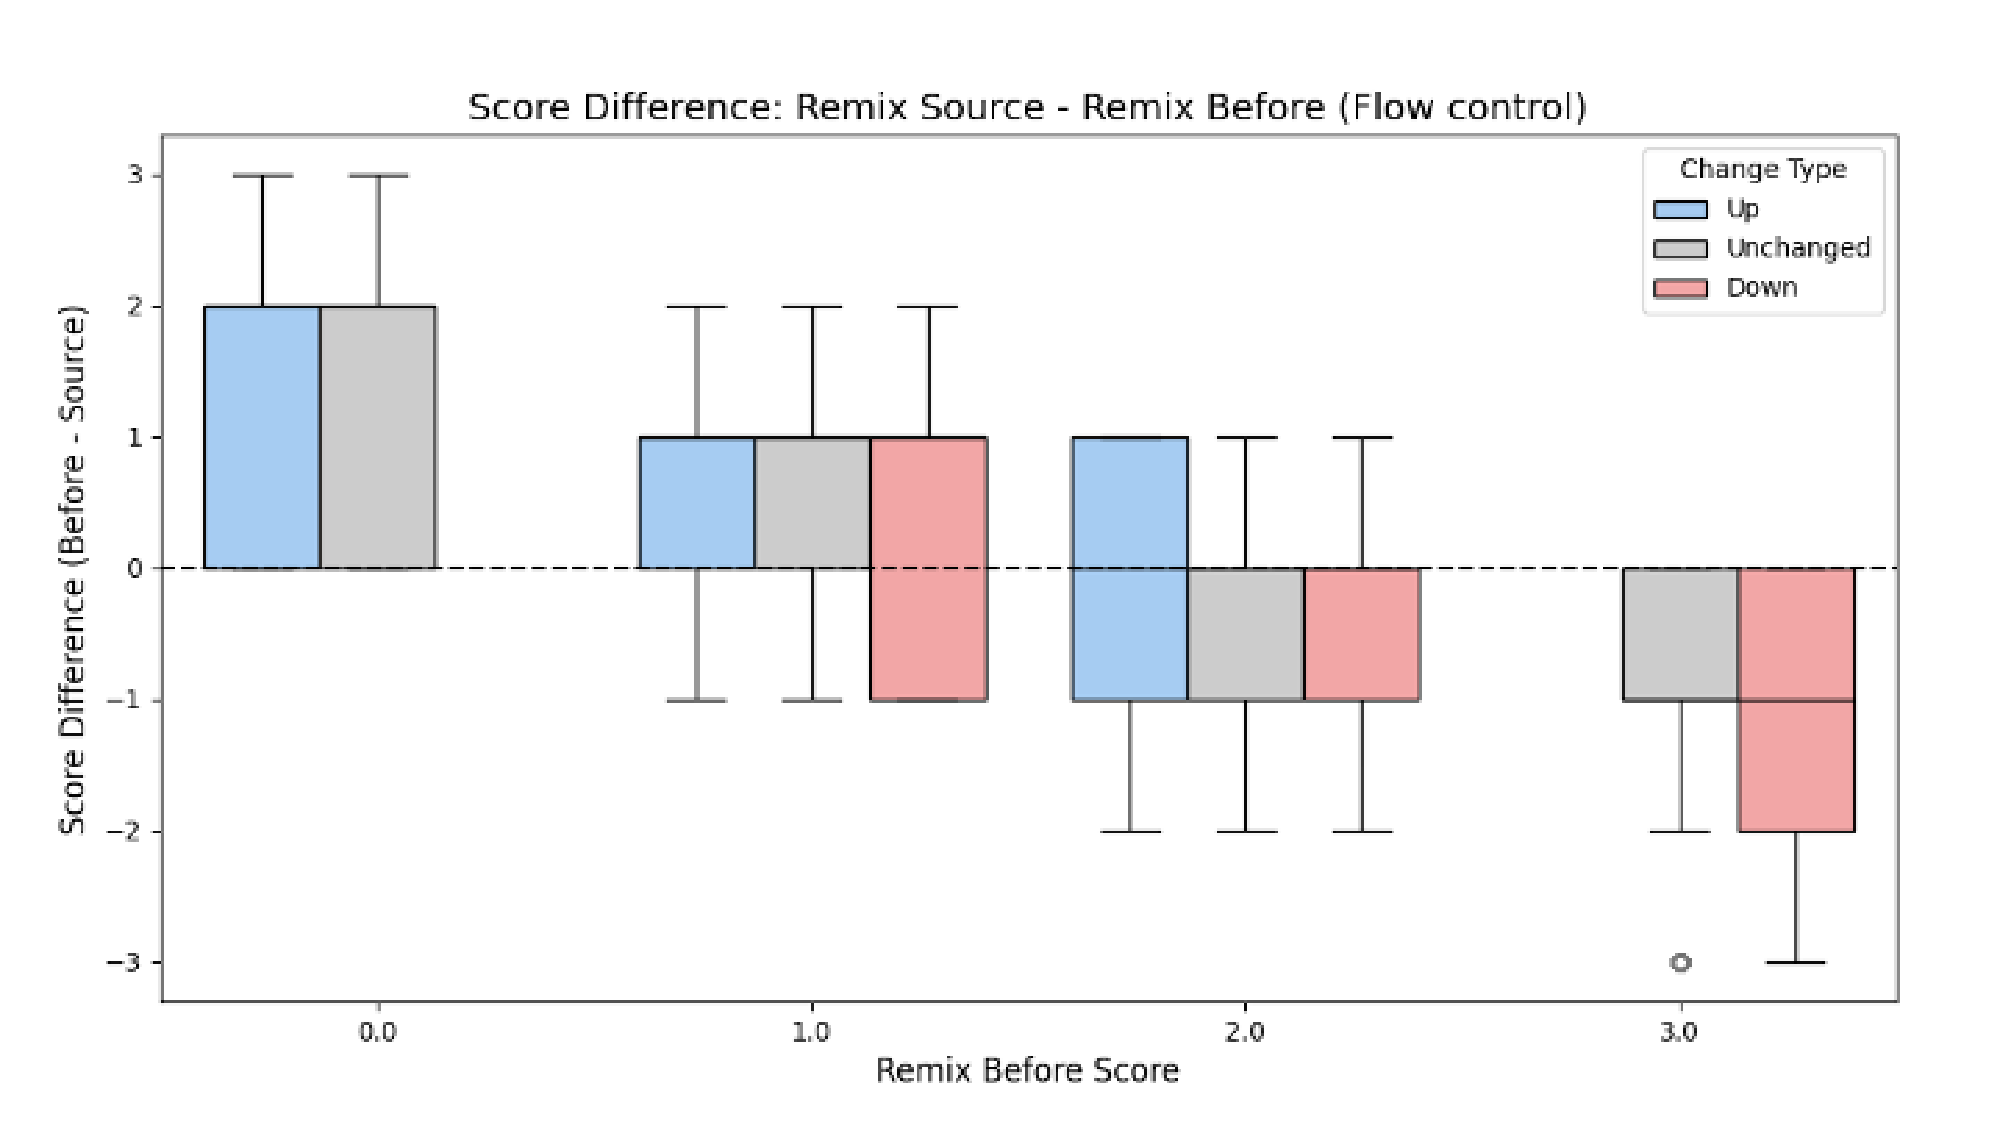
\includegraphics[width=0.7\linewidth]{@BSthesis2024_Horio/BSthesis2024_Horio_fig/Flowcontrol-boxplot.pdf}}
\caption{ユーザのフロー制御スコアごとのリミックス元作品のフロー制御スコア}
\label{fig:Flowcontrol-boxplot}
\end{figure}
%-------------------
%-------------------
\begin{figure}[h]
\centerline{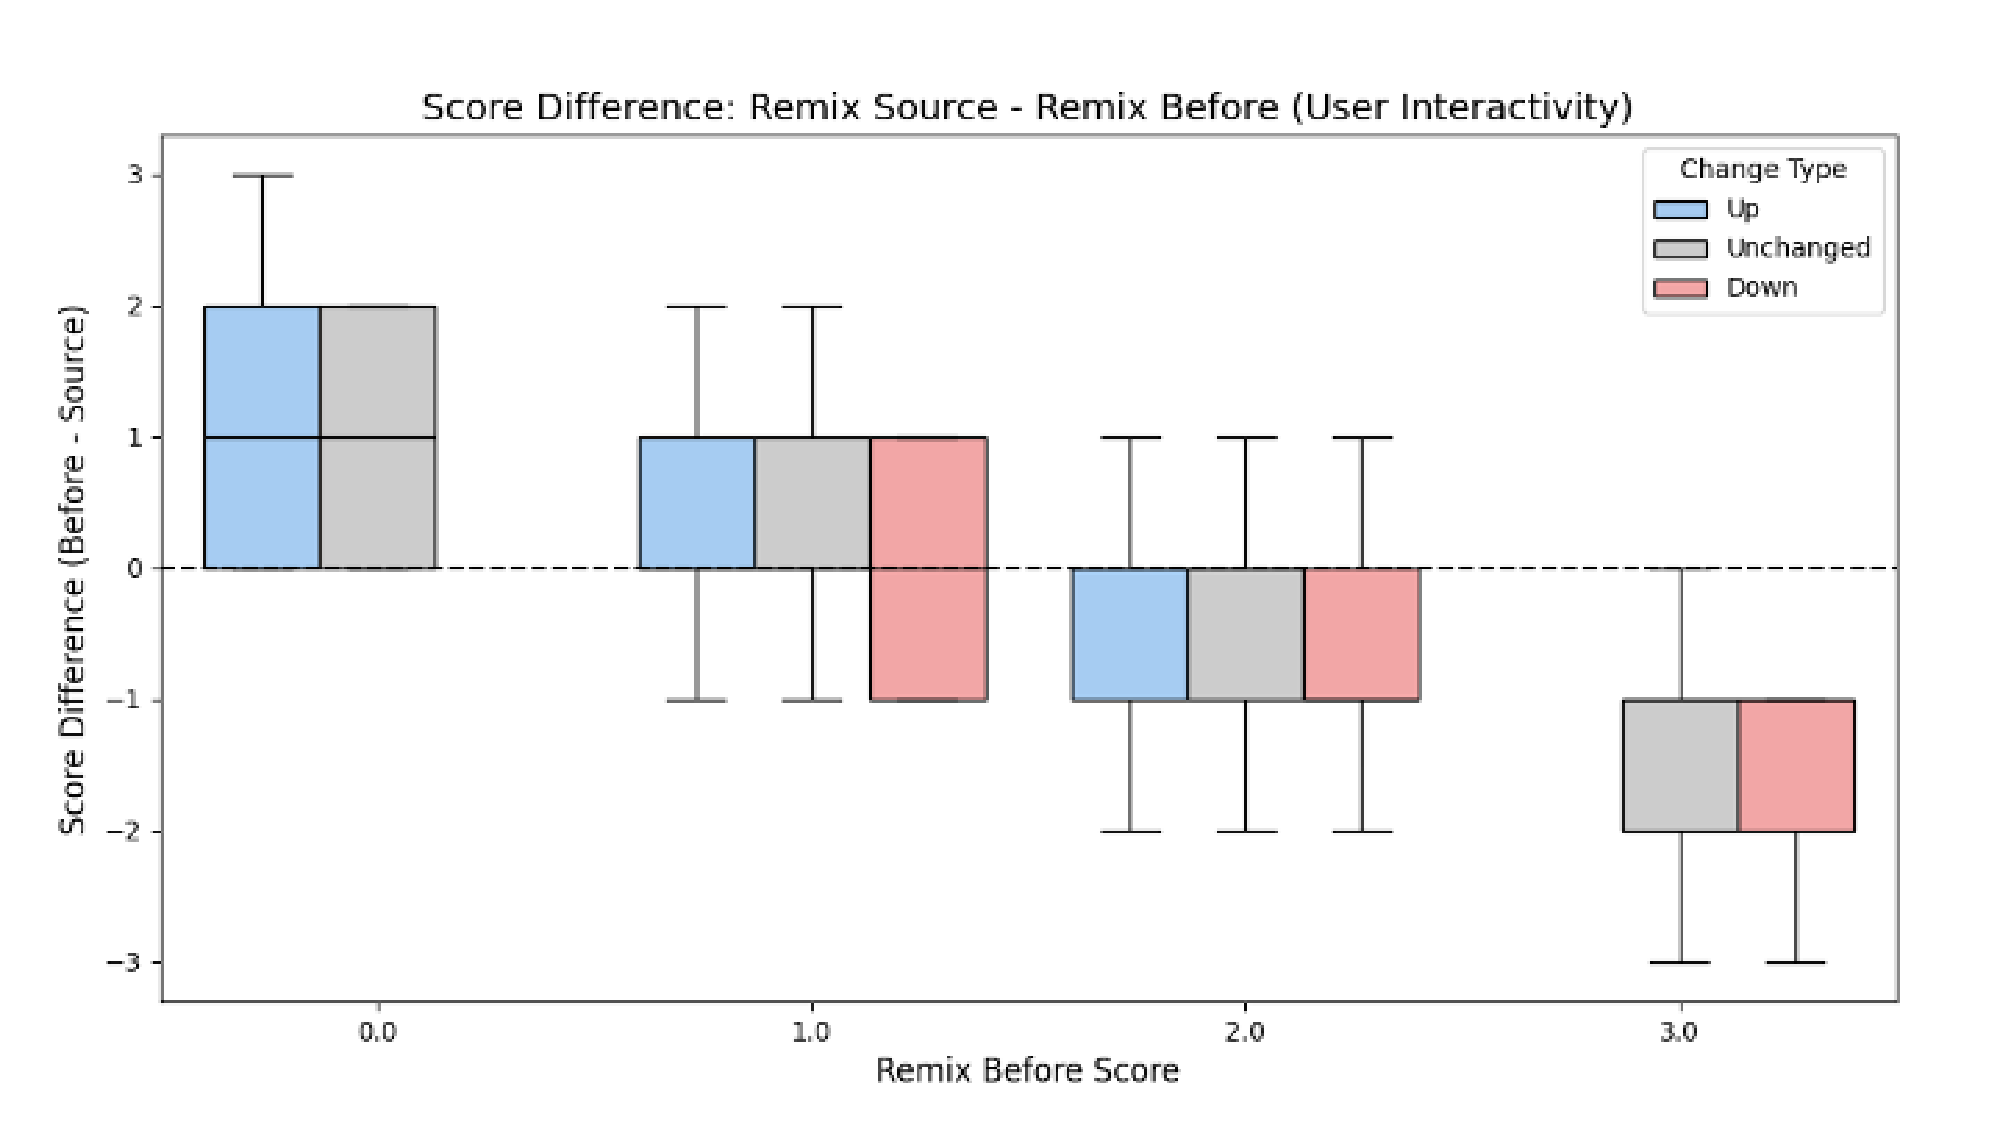
\includegraphics[width=0.7\linewidth]{@BSthesis2024_Horio/BSthesis2024_Horio_fig/UserInteractivity-boxplot.pdf}}
\caption{ユーザのユーザ対話性スコアごとのリミックス元作品のユーザ対話性スコア}
\label{fig:UserInteractivity-boxplot}
\end{figure}
%-------------------
%-------------------
\begin{figure}[h]
\centerline{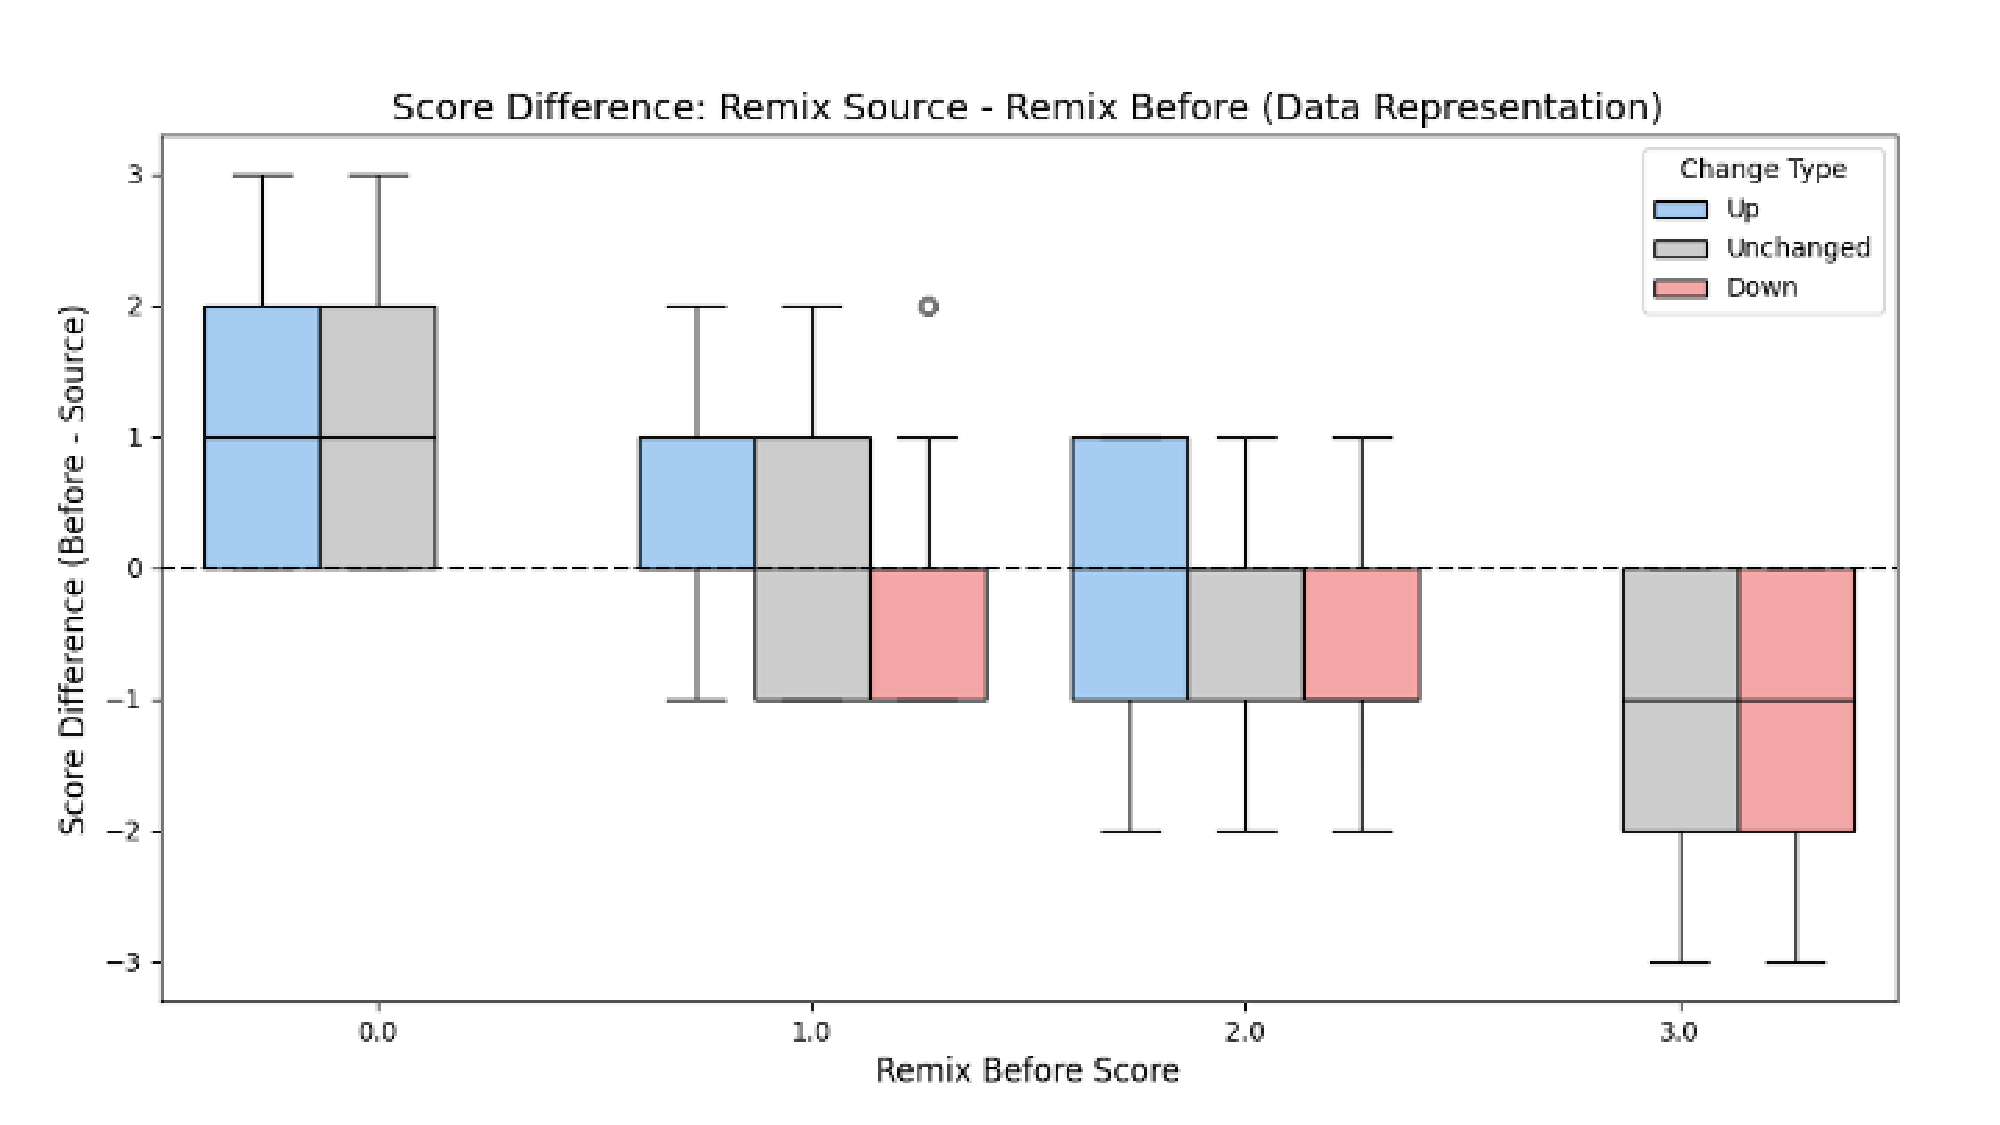
\includegraphics[width=0.7\linewidth]{@BSthesis2024_Horio/BSthesis2024_Horio_fig/DataRepresentation-boxplot.pdf}}
\caption{ユーザのデータ表現スコアごとのリミックス元作品のデータ表現スコア}
\label{fig:DataRepresentation-boxplot}
\end{figure}
%-------------------
\section{考察}

\chapter{RQ2:リミックスによって向上するユーザのCTスコアは,CTスコア概念による傾向があるか?}
\section{概要}

\section{分析手法}
\section{分析結果}
\section{考察}


\chapter{妥当性の脅威}

\section{内的妥当性}
本研究では,ユーザがリミックスにより向上したCTスキルを分析するための設定として,ユーザがリミックス後に制作したオリジナル作品のCTスコアを,リミックス後のユーザのCTスキルとしている.しかし,リミックス後に制作したオリジナル作品のCTスコアは,リミックスだけでなく,オリジナル作品の制作を重ねることで向上する可能性がある.本研究では,リミックス後のユーザのCTスキルをリミックス直後に制作したオリジナル作品3作品のうちCTスコアが最も高い作品とすることにより,脅威を軽減する.

\section{外的妥当性}
本研究ではScratchAPIにより,データセットの取得を行い,リミックス作品とオリジナル作品の判別を行ったが,リミックスを介さずにほかユーザの作品を模倣して制作した作品や,他ユーザがアカウントを使用し制作した作品,他ユーザが支援を行い制作した作品が存在する可能性がある.このような作品がデータセットに混ざっている場合,分析に違いが生じることが考えられる.本研究ではリミックスを行ったことがあるユーザを対象に,多くのデータセットを用意し,合計7,551人のユーザの136,283件の作品を対象にすることにより,脅威となるような作品の影響を軽減する.

\chapter{おわりに}

% 文献を参照する場合には,論文の最後に参考文献として列挙するとともに,
% \verb|\cite|を使って,例えば,
% \begin{quote}
%   文献\cite{latex}によれば…
% \end{quote}
% や,
% \begin{quote}
%   …である\cite{latex2e}.
% \end{quote}
% のように参照する.

% 文献の列挙には,{\tt thebibliography}環境などを用いる\footnote{使い方
% は,この資料のソースを参照.}.

%%%%%%%%%%%%%%%%%%%%%%%%%%%%%%%%%%%%%%%%%%%%%%%%%%%%%%%%%%%%%%%%%%%%%%%%


% 謝辞

\begin{acknowledgements}
感謝します.
\end{acknowledgements}

%%%%%%%%%%%%%%%%%%%%%%%%%%%%%%%%%%%%%%%%%%%%%%%%%%%%%%%%%%%%%%%%%%%%%%%%

%%
%% 参考文献
%%

\bibliographystyle{junsrt}
\bibliography{@BSthesis2024_Horio/BSthesis2024_Horio}

\end{document}

%%%%%%%%%%%%%%%%%%%%%%%%%%%%%%%%%%%%%%%%%%%%%%%%%%%%%%%%%%%%%%%%%%%%%%%%

%%
%% 付録
%%
% \appendix
% 
% \chapter{サンプルプログラム}
% 
% プログラムリストや実行結果など,本論を補足する上で必要と思われるものが
% あれば付録として付ける.
% 
% {
% \footnotesize
% \begin{verbatim}
% #include <stdio.h>
% int main(void)
% {
%     printf("Hello, World!\n");
%     return 0;
% }
% \end{verbatim}
% }

%%%%%%%%%%%%%%%%%%%%%%%%%%%%%%%%%%%%%%%%%%%%%%%%%%%%%%%%%%%%%%%%%%%%%%%%

\end{document}
